\documentclass{standalone}

\usepackage{tikz}
\usetikzlibrary{arrows}
\usetikzlibrary{decorations.pathmorphing,patterns}

\begin{document}

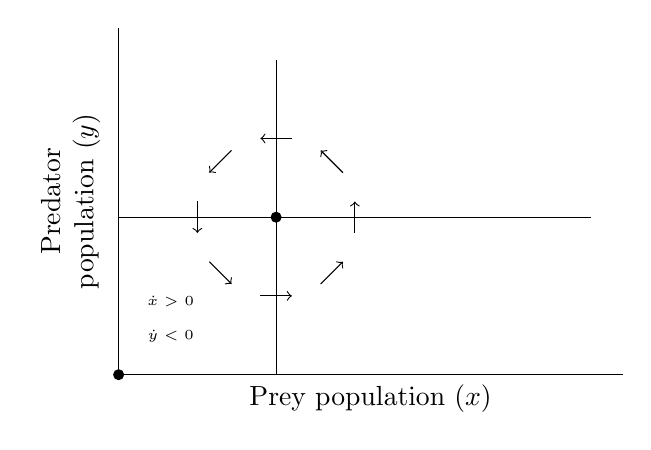
\begin{tikzpicture}[scale=2]
\draw (0,0) -- (3.2,0) node[pos=.5, below]{Prey population ($x$)};  
\draw (0,0) -- (0,2.2) node[pos=.5, sloped, above=2pt]{\begin{tabular}{c} Predator \\ population ($y$)\end{tabular}};
\fill (1,1) circle(1pt);
\fill (0,0) circle(1pt);
\draw (1,0) -- (1,2);
\draw (0,1) -- (3,1);
  \draw[->] (1,.5)+(-.1,0) -- +(0.1,0);
  \draw[<-] (1,1.5)+(-.1,0) -- +(0.1,0); 
  \draw[<-] (.5,1)+(0,-.1) -- +(0,0.1); 
  \draw[->] (1.5,1)+(0,-.1) -- +(0,0.1); 
  \draw[->] (1,1)++(45:.5)+(-45:.1) -- +(135:0.1); 
  \draw[->] (1,1)++(135:.5)+(45:.1) -- +(-135:0.1); 
  \draw[->] (1,1)++(-45:.5)+(-135:.1) -- +(45:0.1); 
  \draw[->] (1,1)++(-135:.5)+(135:.1) -- +(-45:0.1); 
  \draw (1,1)++(-135:.5)node[below left,]{\begin{tabular}{c} \tiny$\dot{x}>0$ \\ \tiny$\dot{y}<0$\end{tabular}};
\end{tikzpicture}


\end{document}

